\documentclass[addpoints]{exam}
\printanswers
\usepackage{listings} % for code insertion https://www.overleaf.com/learn/latex/Code_listing
\usepackage{xcolor, graphicx}

\definecolor{codegreen}{rgb}{0,0.6,0}
\definecolor{codegray}{rgb}{0.5,0.5,0.5}
\definecolor{codepurple}{rgb}{0.58,0,0.82}
\definecolor{backcolour}{rgb}{0.95,0.95,0.92}

\lstdefinestyle{mystyle}{
    commentstyle=\color{codegreen},
    keywordstyle=\color{magenta},
    numberstyle=\tiny\color{codegray},
    stringstyle=\color{codepurple},
    basicstyle=\ttfamily\footnotesize,
    breakatwhitespace=false,
    breaklines=true,
    captionpos=b,
    keepspaces=true,
    numbers=left,
    numbersep=5pt,
    showspaces=false,
    showstringspaces=false,
    showtabs=false,
    tabsize=2
}

\lstset{style=mystyle}

% writes in french the total number of points https://www.overleaf.com/learn/latex/Typesetting_exams_in_LaTeX#Other_languages
\totalformat{Total pour la question \thequestion : \totalpoints points}

\title{Test 1M3 représentation de l'information et enjeux sociaux}
\date{25/01/2023 - 45mn}

\begin{document}

\maketitle

\begin{center}
\fbox{\fbox{\parbox{5.5in}{\centering
\begin{itemize}
\item Utilisez un stylo bleu ou noir, pas de crayon à papier.
\item Pour les questions ouvertes (non QCM) indiquez votre raisonnement de manière \textbf{concise et précise}. Privilégiez des phrases courtes et votre suite d'égalités logiques pour justifier de vos résultats numériques par exemple. Le raisonnement fait partie intégrante de l'évaluation.
\item Vous devez ranger vos téléphones dans vos sacs avant le début du test.
\item Les calculatrices ne sont pas autorisées.
\item Les questions QCM ont une seule réponse correcte possible.
\item Pensez à correctement effecter les conversions octets-Ko \textbf{(1Ko=1024 octets)}.
\item 1 pouce = 2,54cm.
\end{itemize}
}}}
\end{center}

\vspace{5mm}
\makebox[0.75\textwidth]{Nom et prénom:\enspace\hrulefill}
\vspace{5mm}

\begin{center}
\gradetable[h][questions]
\end{center}

\textbf{Commentaire de l'enseignant :}
\makeemptybox{\stretch{1}}

\clearpage

\begin{questions}
\question Images numériques
\droptotalpoints
\begin{parts}
\part[1] Quelle est la \textbf{définition} d'une feuille scannée de largeur 4 pouces, de hauteur 7 pouces en 250dpi ?
\begin{solutionordottedlines}[\stretch{1}]
	Nombre de pixels de large : $4\times 250=1000px$. Nombre de pixels de long : $7\times 250=1750px$. La définition est donc de 1,75 million de pixels (ou mega pixels)
\end{solutionordottedlines}
\part[1] Vous souhaitez imprimer un fichier jpeg contenant une image sur une feuille A4. Quels sont les deux points importants pour obtenir une bonne qualité d'impression de l'image ? Justifiez votre réponse.
\begin{solutionordottedlines}[\stretch{1}]
	Les deux éléments sont la \textbf{définition} et la \textbf{résolution} :
	\begin{itemize}
	\item Une \textbf{image} avec une meilleure définition contient effectivement plus de pixels ce qui permet d'atteindre un niveau de détails plus fin.
	\item L'\textbf{impression} doit être faite avec une bonne résolution. En effet la résolution détermine le nombre de pixels qui seront imprimés sur chaque pouce d'une feuille de papier : une meilleure résolution signifie plus de pixels sur le même nombre de pouces donc une image plus fine.
	\end{itemize}
\end{solutionordottedlines}
\part[3] Complétez le tableau suivant pour donner la taille mémoire occupée par les images de différentes dimensions. Considérez qu'un pixel en niveaux de gris occupe 1 octet, et qu'un pixel en couleur occupe 1 octet par canal de couleur. \textit{Pensez à préciser votre unité}

\begin{table}[h]
	\centering
	\renewcommand{\arraystretch}{2}
	\begin{tabular}[h]{| c | c | c |}
	\hline
	Définition & gris & couleur \\
	\hline
	$200\times 200$ & \fillin[39.1Ko] & \fillin[117.2Ko] \\
	$12\times 14$ & \fillin[168 octets] & \fillin[504 octets] \\
	$720\times 1080$ & \fillin[759.4Ko] & \fillin[2.225Mo] \\
	\hline
	\end{tabular}
	\end{table}
	
\part[2] On considère une image dont la taille mémoire non compressée est de 3Ko. On passe cette image dans un algorithme de compression avec un taux de compression de 25\%. Quel est la taille de cette image \textbf{une fois la compression} appliquée ?
\begin{solutionordottedlines}[\stretch{1}]
	On applique la formule du cours : $taux\_de\_compression = 1-\frac{taille\_compressee}{taille\_non\_compressee}$. Soit $0,25=1-\frac{taille\_compressee}{3072}$. Notez que $3Ko=3\times 1024=3072\ octets$. En manipulant l'équation, on obtient :\\
		$\frac{taille\_compressee}{3072}=0,75$ soit $taille\_compressee=0,75\times 3072=2304\ octets=2,25Ko$. Il était également possible de faire ce calcul sans la conversion en octets et en obtenant directement un résultat en Ko.
\end{solutionordottedlines}
\end{parts}

\clearpage

\question Représentation du son
\droptotalpoints
\begin{parts}
\part[2] La fréquence d'échantillonnage représente \fillin[l'intervalle de temps entre deux mesures][3in] d'une onde.
\part[1] Une plus grande \textbf{profondeur d'échantillonnage} permet généralement d'avoir :
\begin{checkboxes}
    \choice Une moins bonne qualité audio à la reconstruction
    \choice Une qualité audio identique
    \CorrectChoice Une meilleure qualité audio à la reconstruction
\end{checkboxes}
\part[3] Sur le diagramme suivant, ajoutez les points de capture de l'onde sonore pour une fréquence d'échantillonnage de 200Hz et une profondeur d'échantillonnage de 3 bits.
\ifprintanswers
    \begin{figure}[h]
    \centering
    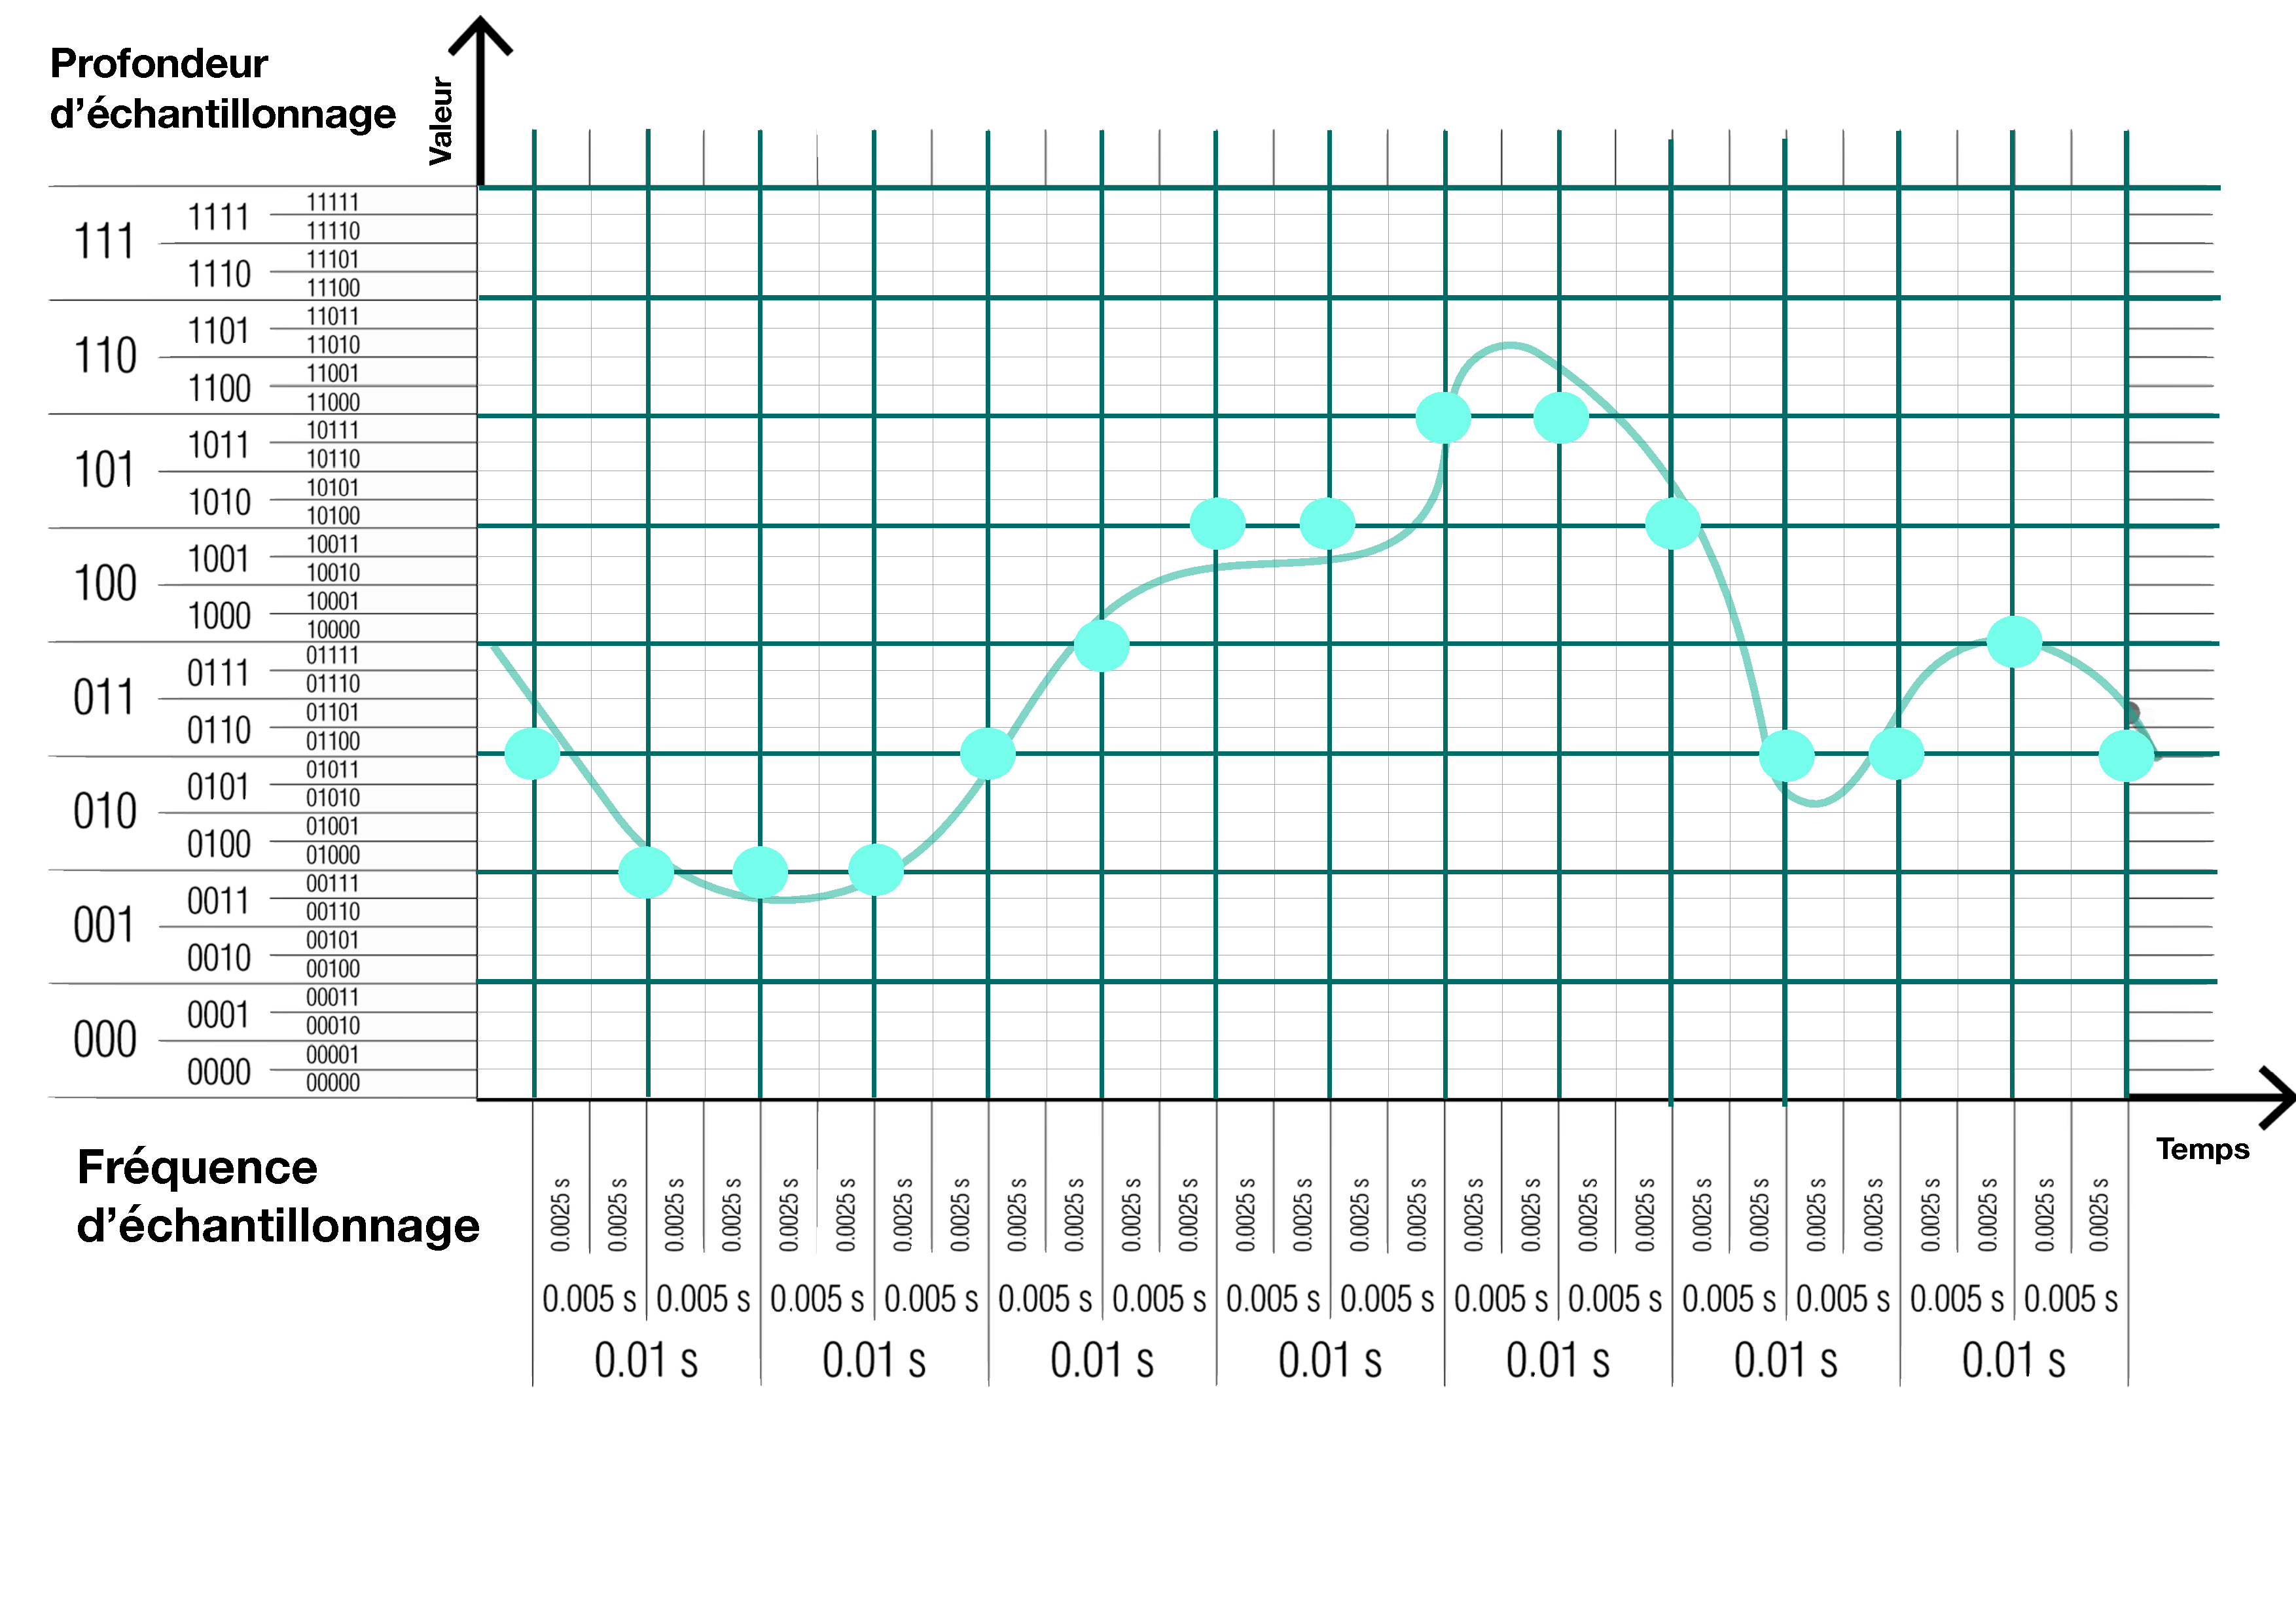
\includegraphics[width=\linewidth]{Exercice Echantillonnage - correction.pdf}
    \end{figure}
\else
	\begin{figure}[h]
    \centering
    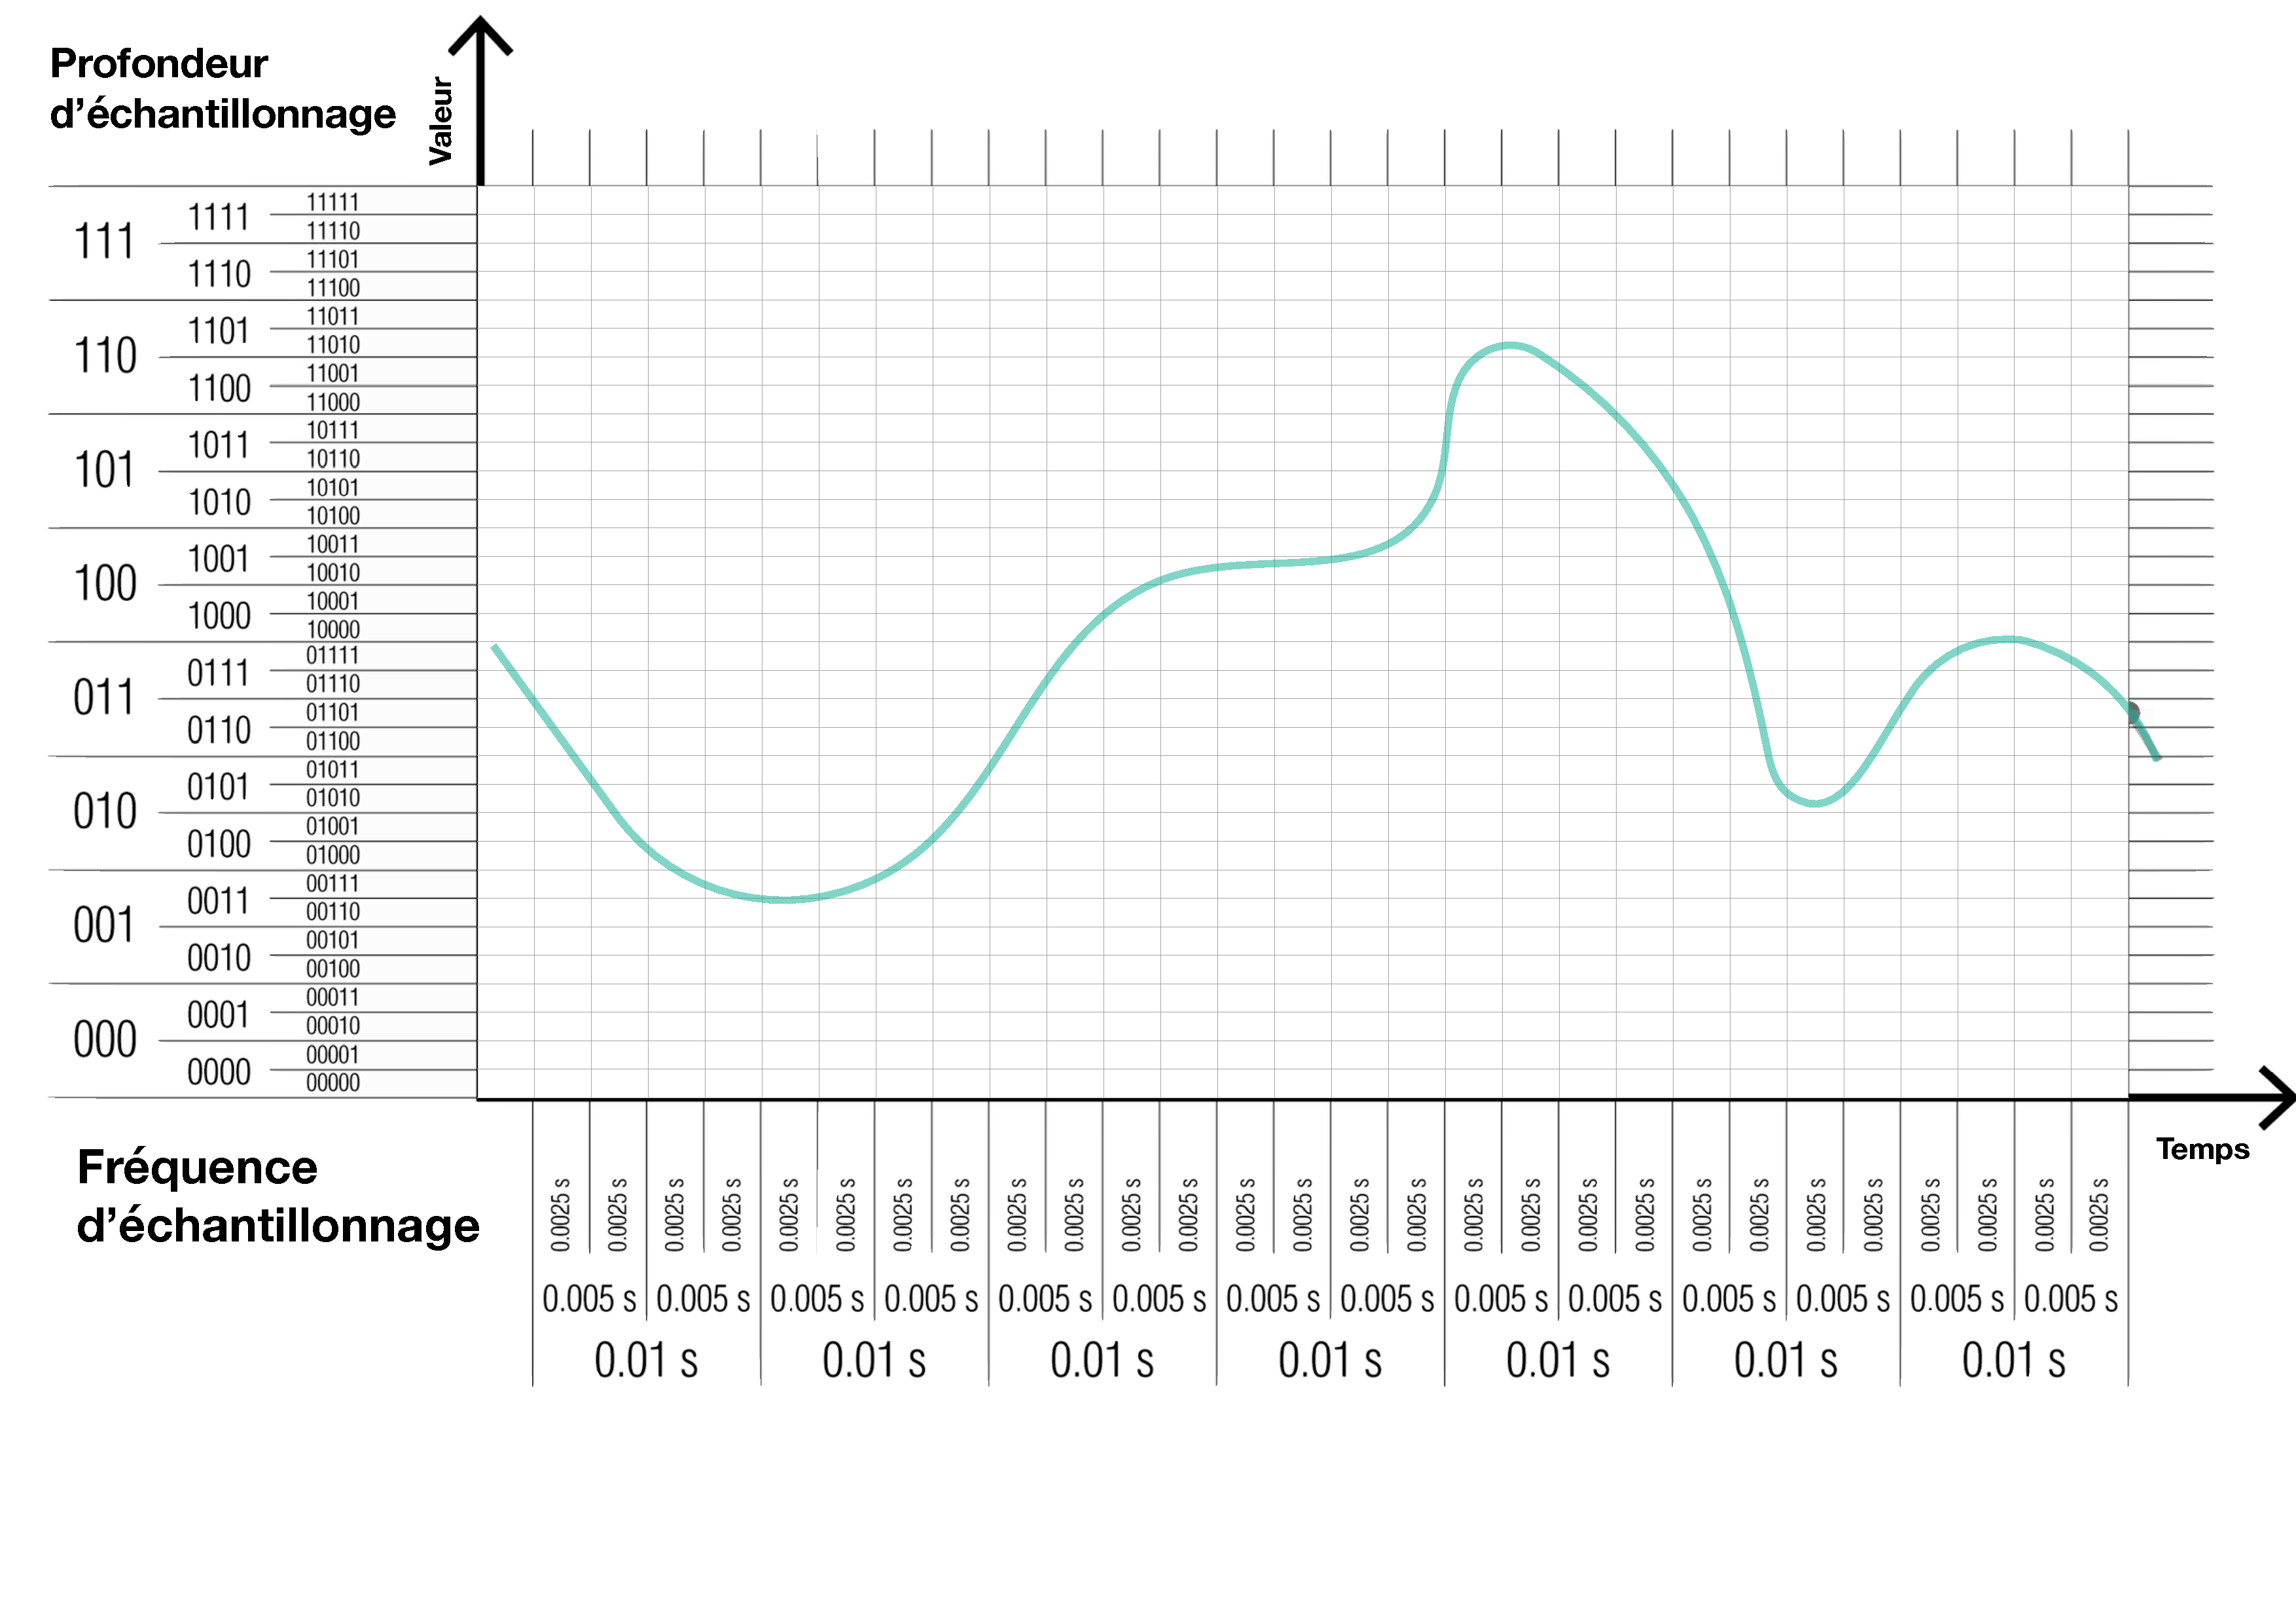
\includegraphics[width=\linewidth]{Exercice Echantillonnage.pdf}
	\end{figure}
\fi
\end{parts}

\question Redondance
\droptotalpoints
\begin{parts}
\part[2] Votre ami·e vous envoie un message binaire en utilisant la technique du \textbf{bit de parité}. Ce message, très court, tient sur sur une seule lettre codée sur 8 bits. Vous recevez donc les 9 bits suivant : $001110001$. Pouvez vous dire si le message transmis contient une erreur ? Précisez votre raisonnement.
\begin{solutionordottedlines}[\stretch{1}]
	On calcul le bit de parité que devraient avoir les 8 premiers bits : $0+0+1+1+1+0+0+0=3$ qui est impair, donc le bit de parité devrait être 1, or le neuvième bit est bien 1 : ce message ne contient pas une erreur sur un bit.
\end{solutionordottedlines}
\end{parts}

\clearpage

\question Economie du numérique
\droptotalpoints
\begin{parts}
\part[2] Vous avez vu en classe la notion d'\textbf{effet de réseau}. Expliquez en quoi cela consiste et détaillez l'exemple d'une plateforme que vous connaissez qui en bénéficie.
\begin{solutionordottedlines}[\stretch{1}]
	L'effet de réseau est une mécanique qui, dans le cadre des plateformes numérique, consiste en l'accroit de l'intérêt d'une plateforme par l'augmentation de son nombre d'utilisateur-trice-s. Ainsi, plus il y a de personne qui utilisent la plateforme, plus celle-ci gagne en intérêt et plus il y aura d'utilisateur·trice·s attiré·e·s. 
	
	C'est typiquement une mécanique dont les réseaux sociaux (Instagram, BeReal) bénéficient : l'intérêt de ces plateformes résidant dans l'interaction sociale, plus il y a de personnes présentes plus l'interaction sociale sera forte et fera gagner de l'intérêt à la plateforme.
\end{solutionordottedlines}

\part[1] Dans le cas de Google, l'utilisation des données personnelles est particulièrement lucrative (rapporte de l'argent) car (cochez la réponse qui permet la plus importante source de revenus à Google):
\begin{checkboxes}
\choice Il est possible de les revendre à Facebook
\CorrectChoice Il est possible de proposer aux annonceurs des emplacements d'annonces ciblées
\choice Il est possible de proposer aux annonceur d'acheter directement ces données
\choice Il est ensuite possible de faire acheter des produits Google aux utilisateur·trice·s.
\end{checkboxes}

\begin{solution}
En effet, Google a tout intérêt à ne pas vendre ces données à Facebook, car c'est son concurrent sur ce domaine (Voir TP GAFAM) ! 

De même, les annonceurs n'ont pas d'intérêt direct à acheter ces données : cela a un coût et ne permet pas directement de vendre des produits. De puis la manipulation des données requiert un expertise qu'il y a tout intérêt à laisser à un acteur comme Google (Voir cours enchères du numérique). 

Enfin, la très grande majorité des produits Google sont gratuits (Gmail, le moteur de recherche Google, Google Chrome, Youtube, ...). L'intérêt de Google est de permettre au plus grand nombre d'utiliser ces produits pour accumuler des données et les utiliser pour des emplacements publicitaires ciblés, intéressants pour les annonceurs, pas de vendre ces produits aux particuliers (Voir TP GAFAM et cours enchères du numérique).
\end{solution}

\vspace{\stretch{2}}
\end{parts}
\end{questions}
\end{document}